\documentclass[12pt]{article}

\usepackage{sbc-template}
\usepackage{graphicx,url,booktabs}
\usepackage[utf8]{inputenc}
\usepackage[brazil]{babel}
\graphicspath{{figs/}{../evidencias/}}

\sloppy

\title{Istio na prática: mTLS, controle de tráfego e observabilidade\\
em microsserviços Go no Kubernetes}

\author{Gustavo Parcianello Cardona\inst{1}, Danielle Hikaru Toma\inst{1}}

\address{Escola Politécnica -- Universidade do Vale do Rio dos Sinos (UNISINOS)\\
  São Leopoldo -- RS -- Brasil
  \email{gcardona@edu.unisinos.br, dtoma@edu.unisinos.br}
}

\begin{document}

\maketitle

\begin{resumo}
  Este artigo implementa e mede um protótipo da malha de serviços Istio
  (modo sidecar) no Azure Kubernetes Service. A mesma cadeia de serviços em Go
  roda em três modos: HTTP puro, as mesmas funções de segurança e resiliência
  escritas no código da aplicação, e Istio. Os modos B e C barram clientes não
  autorizados e limitam a latência de uma dependência lenta da mesma forma. O
  modo C usa 31 linhas de YAML em vez de 227 linhas de Go e scripts, e ainda
  entrega métricas, logs, traces e rotação automática de certificados. O mTLS
  escrito na aplicação acrescentou menos de 0,1~ms; o custo do Istio veio dos
  proxies: cerca de 1~ms por salto com baixa concorrência, cerca de 46~ms fim a
  fim com 32 conexões em nós de 2 vCPU e cerca de seis vezes mais memória. Com
  20 conexões fechadas, a vazão do modo C ficou abaixo da dos outros modos e
  subiu cerca de 75\% quando o rastreamento passou de 100\% para 1\% e o
  registro de acesso foi desligado.
\end{resumo}

\section{Introdução}

Em uma arquitetura de microsserviços, toda chamada entre serviços atravessa a
rede e precisa das mesmas proteções: cifragem e autenticação mútua, decisão
sobre quem pode chamar quem, limites de tempo e retentativas diante de falhas,
e visibilidade sobre volume, erros e latência de cada salto. Sem uma camada
comum, cada equipe reescreve essas funções em cada serviço e em cada
linguagem~\cite{redhat,flinders}.

Uma \emph{service mesh} move essas funções para a infraestrutura. No Istio, um
proxy Envoy é colocado ao lado de cada instância da aplicação (o
\emph{sidecar}) e um plano de controle, o \texttt{istiod}, distribui
configuração e certificados~\cite{istio-arch}. No Grau A deste trabalho o
Istio foi escolhido e estudado como middleware. Este artigo, do Grau B,
implementa um protótipo, implanta-o em um cluster Kubernetes real e mede o que
o Istio facilita e quanto ele custa.

A comparação é feita em três modos sobre o mesmo binário Go: (A) HTTP puro,
sem as funções; (B) as funções escritas na própria aplicação; e (C) Istio, com
as funções desligadas no código. O modo B permite separar o custo das funções
do custo de executá-las em um proxy, o que uma comparação apenas entre Istio e
HTTP puro não permite.

As contribuições são: (i) um protótipo reproduzível em Go, Kubernetes e Istio,
com scripts de infraestrutura, carga e coleta; (ii) medições de segurança,
latência, recursos, resiliência, circuit breaker e divisão de tráfego nos três
modos; e (iii) evidências de observabilidade coletadas no cluster com Kiali,
Prometheus, Grafana, Loki e Jaeger.

\section{Fundamentação}

\subsection{Istio e o modo sidecar}

O Istio separa um plano de dados, formado pelos proxies Envoy, de um plano de
controle, o \texttt{istiod}~\cite{istio-arch}. Quando um \emph{namespace} recebe
o rótulo \texttt{istio-injection=enabled}, um \emph{webhook} de admissão do
\texttt{istiod} acrescenta a cada novo pod um contêiner \texttt{istio-proxy} e
um contêiner de inicialização, o \texttt{istio-init}. Este cria regras
\texttt{iptables} que desviam todo o tráfego de entrada (porta 15006) e de
saída (porta 15001) para o Envoy, de modo que a aplicação continua falando
HTTP simples sem perceber o proxy. O \texttt{istiod} envia a cada Envoy, pelo
protocolo xDS, os \emph{listeners}, rotas, \emph{clusters} e \emph{endpoints}
que ele deve conhecer.

\subsection{Identidade e mTLS}

Cada \emph{workload} recebe uma identidade no formato SPIFFE, derivada da sua
\emph{service account}, por exemplo
\url{spiffe://cluster.local/ns/mesh/sa/frontend}, gravada em um certificado
X.509 de curta duração (24 horas por padrão) e renovado automaticamente pelo
\texttt{istiod}. Entre dois sidecars, o Istio estabelece TLS mútuo (mTLS)
automaticamente. A política \texttt{PeerAuthentication} define se conexões sem
mTLS são aceitas (\texttt{PERMISSIVE}) ou recusadas (\texttt{STRICT}), e a
\texttt{AuthorizationPolicy} decide, a partir da identidade autenticada, quem
pode chamar cada serviço. Esse modelo segue os princípios de arquitetura de
confiança zero~\cite{rose2020}.

\subsection{Controle de tráfego e observabilidade}

Regras declaradas em \texttt{VirtualService} e \texttt{DestinationRule}
permitem dividir tráfego entre versões por peso, impor tempo limite e
retentativas, limitar conexões e ejetar instâncias com falhas
(\emph{outlier detection}). Como todo tráfego passa pelos proxies, eles também
emitem métricas no formato Prometheus, registros de acesso e \emph{spans} de
rastreamento distribuído, sem instrumentação na aplicação. A aplicação precisa
apenas repassar os cabeçalhos de rastreamento.

\section{Trabalhos relacionados}

A documentação do Istio publica medições de desempenho e escalabilidade do
plano de dados~\cite{istio-perf}. Zhu et al. medem o custo de latência e de CPU
do Envoy como sidecar e atribuem a maior parte dele ao processamento do
protocolo HTTP no proxy~\cite{zhu2023}. Sedghpour et al. estudam políticas de
gerenciamento de tráfego (retentativas e circuit breaker) em malhas de serviço
e seu efeito sobre a latência sob falhas~\cite{sedghpour2022}. Bremler-Barr et
al. comparam Istio, Istio \emph{ambient}, Linkerd e Cilium com mTLS
obrigatório e encontram no Istio em modo sidecar o maior aumento de latência e
de uso de recursos~\cite{barr2025}. Duque et al. avaliam qualitativamente o
gerenciamento de tráfego em nuvem de borda~\cite{duque2022}. Alternativas como
Linkerd~\cite{linkerd}, Cilium~\cite{cilium} e o modo \emph{ambient} do
Istio~\cite{istio-ambient} reduzem o custo por pod com proxies mais leves ou
compartilhados por nó.

Este trabalho compara o Istio não só com HTTP puro, mas também com as mesmas
funções implementadas na aplicação, no mesmo ambiente e com a mesma carga, o
que separa o custo da função do custo do proxy.

\section{Protótipo e arquitetura}

O protótipo é uma cadeia de três serviços em Go 1.22, escrita apenas com a
biblioteca padrão: \texttt{frontend} chama \texttt{catalog} (versões v1 e v2),
que chama \texttt{inventory}. Cada requisição atravessa três saltos. Uma única
imagem de contêiner é usada em todos os modos; o comportamento muda apenas por
variáveis de ambiente e pelo rótulo do \emph{namespace}
(Tabela~\ref{tab:modos}).

\begin{table}[ht]
\centering
\caption{Os três modos comparados.}
\label{tab:modos}
\small
\begin{tabular}{llp{7cm}}
\toprule
Modo & Namespace & O que faz as funções \\
\midrule
A (HTTP puro) & \texttt{plain} & nada (linha de base) \\
B (no código) & \texttt{applib} & código Go: mTLS, retry, timeout, circuit breaker, métricas \\
C (Istio) & \texttt{mesh} & sidecar Envoy, configurado por YAML \\
\bottomrule
\end{tabular}
\end{table}

No modo B, o código acrescenta: mTLS com \texttt{crypto/tls}, exigindo
certificado do cliente e autorizando pelo CN; uma autoridade certificadora e
certificados gerados por script e montados como \emph{Secrets}, sem rotação;
tempo limite total e por tentativa, retentativas, um \emph{circuit breaker} por
falhas consecutivas e um limite de requisições simultâneas; e um
\emph{endpoint} \texttt{/metrics} com contadores e histograma de latência. Essas
funções têm testes unitários. No modo C, o mesmo binário roda com tudo isso
desligado, e as funções equivalentes são declaradas em
\texttt{PeerAuthentication}, \texttt{AuthorizationPolicy}, \texttt{VirtualService}
e \texttt{DestinationRule}.

A infraestrutura é um cluster Azure Kubernetes Service (Kubernetes 1.36) na
região Brazil South, com três nós de 2 vCPU: um nó de sistema (onde ficam
\texttt{istiod} e as ferramentas de observabilidade), um nó de aplicação, que
recebe os serviços dos três modos, e um nó de carga, que recebe o gerador de
carga, para que ele não dispute CPU com os serviços medidos. Foi usado o Istio
1.26.0 no perfil \texttt{default}, com Prometheus, Grafana, Kiali, Jaeger e
Loki (com coleta pelo Grafana Alloy). A carga foi gerada com o
fortio~1.69.5~\cite{fortio}.

\section{Metodologia de testes}

A Tabela~\ref{tab:cenarios} lista os cinco cenários. Nos testes de latência,
os três modos são intercalados dentro de cada rodada para diluir variações do
ambiente, e cada valor reportado é a mediana de três rodadas de 30~s. O
consumo de CPU e memória foi amostrado com \texttt{kubectl top} no meio de cada
rodada, somando apenas os pods da cadeia (incluindo os sidecars em C). Nos
testes de resiliência, a própria aplicação injeta a falha nos três modos (o
\texttt{inventory} atrasa 2~s em 50\% das chamadas), e a política é a mesma em
B e C: tempo limite total de 1~s e uma retentativa com limite de 500~ms. Todas
as medições do modo C usaram rastreamento em 100\% das requisições e registro
de acesso ligado, necessários para as evidências de observabilidade; o teste
de vazão do modo C foi repetido depois com a telemetria no padrão do Istio.

\begin{table}[ht]
\centering
\caption{Cenários, parâmetros e métricas.}
\label{tab:cenarios}
\small
\begin{tabular}{p{2.6cm}p{6.6cm}p{3.6cm}}
\toprule
Cenário & Parâmetros & Métricas \\
\midrule
Latência e recursos & 50 e 500 req/s; 1 e 32 conexões; 3 rodadas de 30~s & p50, p90, p99, CPU, RAM \\
Resiliência & 50 req/s, 64 conexões, 30~s; falha de 2~s em 50\%; timeout 1~s e 1 retry de 500~ms & média, p99, \% de sucesso \\
Circuit breaker e vazão & 20 conexões sem limite de taxa, 10~s, com e sem o limite; no modo C, também 3 rodadas de 20~s com rastreamento em 100\% e em 1\% & req/s, \% de respostas 503 \\
Segurança & chamadas sem credencial, com credencial e com identidade errada & código HTTP \\
Divisão de tráfego & pesos 100/0, 90/10, 50/50, 0/100 entre v1 e v2; 200 req. & requisições por versão \\
\bottomrule
\end{tabular}
\end{table}

\section{Resultados}

\subsection{Segurança}

A Tabela~\ref{tab:seg} resume quem conseguiu chamar o quê. No modo A, qualquer
pod do cluster alcança qualquer serviço. Em B, um cliente sem certificado não
completa o \emph{handshake}, e um cliente com certificado válido, mas CN
diferente de \texttt{frontend}, recebe 403 do \texttt{catalog}. Em C, com
\texttt{PeerAuthentication} em modo \texttt{STRICT}, um pod fora da malha tem a
conexão recusada, e a \texttt{AuthorizationPolicy} devolve 403 a qualquer
\emph{service account} que não seja a do \texttt{frontend}. O certificado do
sidecar do \texttt{frontend} trazia a identidade
\texttt{spiffe://cluster.local/ns/mesh/sa/frontend} e validade de 24 horas.

\begin{table}[ht]
\centering
\caption{Resultado dos testes de segurança (código HTTP ou recusa da conexão).}
\label{tab:seg}
\small
\begin{tabular}{llll}
\toprule
Teste & A & B & C \\
\midrule
Cliente sem credencial & 200 & recusada & recusada \\
Cliente com credencial & 200 & 200 & 200 \\
Identidade errada $\rightarrow$ \texttt{catalog} & 200 & 403 & 403 \\
Rotação de certificados & -- & manual, sem rotação & automática (24~h) \\
\bottomrule
\end{tabular}
\end{table}

\subsection{Latência e recursos}

A Tabela~\ref{tab:lat} e a Figura~\ref{fig:lat} mostram a latência fim a fim.
O modo B fica praticamente igual ao A em todos os casos: com uma conexão, o p50
passa de 1,41~ms para 1,48~ms a 50~req/s e não muda a 500~req/s. O mTLS feito
na aplicação, com conexões reaproveitadas, acrescentou menos de 0,1~ms.

O modo C acrescenta cerca de 2 a 3~ms no p50 com uma conexão, aproximadamente
1~ms por salto. Com 32 conexões a diferença aumenta: o p50 vai de cerca de
8~ms (A e B) para cerca de 46~ms, e o p99 chega a 101--130~ms. A 500~req/s com
uma conexão, o modo C entregou 309~req/s, porque cada requisição levava cerca
de 3,2~ms e uma conexão sequencial não comporta 500 por segundo.

\begin{table}[ht]
\centering
\caption{Latência fim a fim (ms, mediana de 3 rodadas) e recursos da cadeia.}
\label{tab:lat}
\small
\begin{tabular}{lrrrrrrrr}
\toprule
Modo & req/s & con. & obtidas & p50 & p90 & p99 & CPU (m) & RAM (Mi) \\
\midrule
A & 50 & 1 & 50 & 1,41 & 1,93 & 2,98 & 9 & 29 \\
B & 50 & 1 & 50 & 1,48 & 1,95 & 3,00 & 93 & 33 \\
C & 50 & 1 & 50 & 4,61 & 6,26 & 9,54 & 271 & 192 \\
\midrule
A & 50 & 32 & 50 & 7,53 & 10,40 & 14,30 & 5 & 28 \\
B & 50 & 32 & 50 & 8,54 & 12,97 & 25,96 & 18 & 30 \\
C & 50 & 32 & 50 & 45,94 & 59,55 & 101,31 & 40 & 193 \\
\midrule
A & 500 & 1 & 500 & 0,79 & 1,31 & 2,39 & 13 & 30 \\
B & 500 & 1 & 500 & 0,81 & 1,45 & 2,54 & 11 & 31 \\
C & 500 & 1 & 309 & 2,91 & 4,41 & 7,42 & 48 & 191 \\
\midrule
A & 500 & 32 & 500 & 7,72 & 11,38 & 20,26 & 34 & 29 \\
B & 500 & 32 & 500 & 8,40 & 12,11 & 20,95 & 74 & 29 \\
C & 500 & 32 & 499 & 45,76 & 75,57 & 130,40 & 165 & 192 \\
\bottomrule
\end{tabular}
\end{table}

\begin{figure}[ht]
\centering
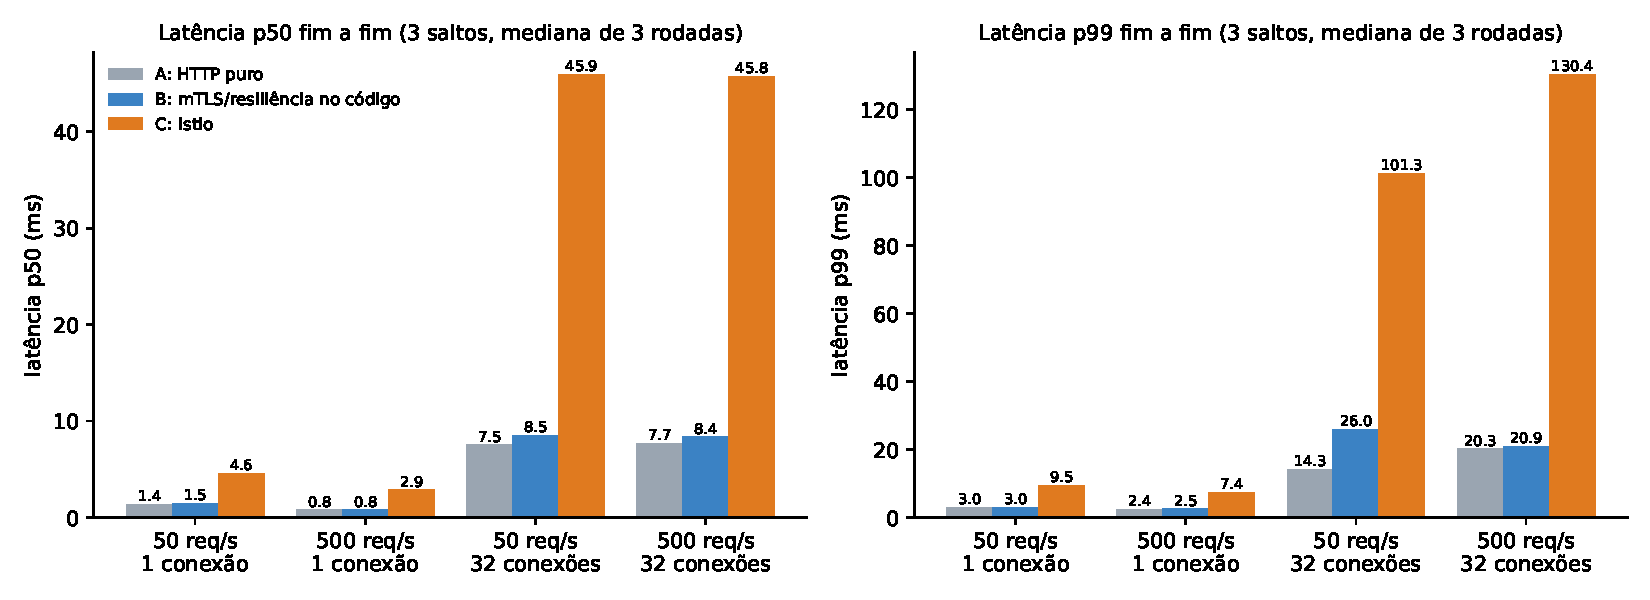
\includegraphics[width=\textwidth]{cmp_latencia.pdf}
\caption{Latência p50 e p99 fim a fim nos três modos.}
\label{fig:lat}
\end{figure}

A memória é a diferença mais estável: cerca de 30~Mi na cadeia em A e B contra
cerca de 190~Mi em C, porque cada sidecar ocupa de 35 a 45~Mi. As amostras de
CPU do \texttt{kubectl top} oscilaram entre rodadas (por exemplo, 93~m em B
com 50~req/s e uma conexão, contra 11~m a 500~req/s) e devem ser lidas apenas
como ordem de grandeza: a 500~req/s com 32 conexões, C usou cerca de 165~m
contra 34~m em A e 74~m em B.

\subsection{Resiliência}

Sem política de resiliência, os três modos esperam os 2~s da falha: a média
sobe para cerca de 1~s e o p99 para cerca de 2~s (Tabela~\ref{tab:res} e
Figura~\ref{fig:res}). Com tempo limite de 1~s e uma retentativa, B e C cortam
a média pela metade (cerca de 500~ms) e limitam o p99 a 1,26~s e 1,07~s. B
obteve 74\% de sucesso e C, 76\%, perto dos 75\% esperados: com uma
retentativa, a requisição só falha se as duas tentativas caírem na metade
lenta ($1 - 0{,}5^2 = 0{,}75$). As requisições que falham recebem 504 em cerca
de 1~s, em vez de esperar os 2~s. O modo A só teria essa política com mudanças
no código.

\begin{table}[ht]
\centering
\caption{Resiliência com o \texttt{inventory} atrasando 2~s em 50\% das chamadas.}
\label{tab:res}
\small
\begin{tabular}{llrrrr}
\toprule
Modo & Fase & média (ms) & p50 (ms) & p99 (ms) & sucesso \\
\midrule
A & sem falha & 14 & 14 & 29 & 100\% \\
A & com falha & 970 & 13 & 2015 & 100\% \\
B & sem falha & 16 & 15 & 31 & 100\% \\
B & com falha & 996 & 16 & 2021 & 100\% \\
B & falha + política & 532 & 510 & 1256 & 74\% \\
C & sem falha & 96 & 87 & 232 & 100\% \\
C & com falha & 1022 & 140 & 2132 & 100\% \\
C & falha + política & 495 & 319 & 1072 & 76\% \\
\bottomrule
\end{tabular}
\end{table}

\begin{figure}[ht]
\centering
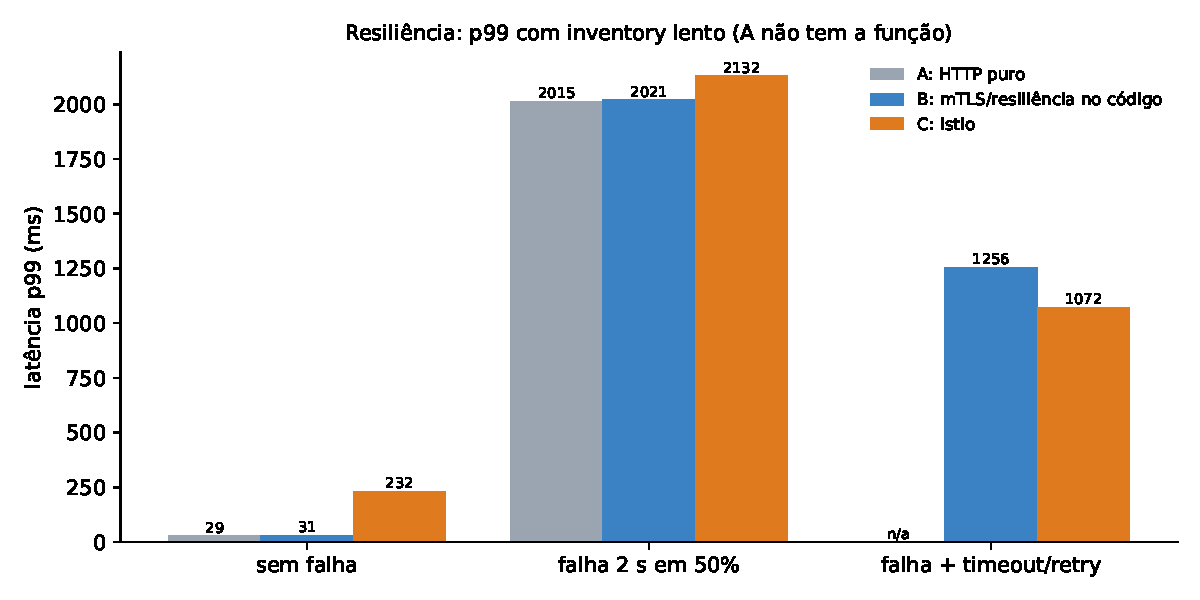
\includegraphics[width=0.8\textwidth]{cmp_resiliencia.pdf}
\caption{Latência p99 com o \texttt{inventory} lento, antes e depois da política.}
\label{fig:res}
\end{figure}

\subsection{Circuit breaker e vazão}

Com 20 conexões e sem limite de taxa, a cadeia atingiu cerca de 3.800~req/s em
A, 3.450~req/s em B e 560~req/s em C. Com o limite ligado (em B, no máximo duas
chamadas simultâneas e abertura do circuito após uma falha; em C, uma
\texttt{DestinationRule} com \texttt{maxConnections: 1} e \emph{outlier
detection}), 66\% das requisições em B e 89\% em C foram rejeitadas
imediatamente com 503, protegendo o serviço de cima.

O valor de C depende do modo de teste e da telemetria. O fortio usa conexões
fechadas: cada uma só envia a próxima requisição depois da resposta, de modo
que a vazão é aproximadamente o número de conexões dividido pela latência. O
teste do modo C foi repetido com três rodadas de 20~s em cada configuração de
telemetria (Tabela~\ref{tab:vazao}). Com o rastreamento em 100\% e o registro
de acesso ligados, como nas coletas de evidências, a cadeia atingiu cerca de
336~req/s, com mediana de 56~ms; com o rastreamento em 1\%, valor padrão do
Istio, e sem registro de acesso, atingiu cerca de 597~req/s, com mediana de
31~ms, cerca de 75\% a mais. O nó de aplicação ficou abaixo de 60\% de CPU,
segundo o \texttt{kubectl top}, de modo que a vazão foi limitada pela latência
de cada requisição, com CPU de sobra. A diferença entre os 560~req/s da
primeira medição e os 336~req/s da repetição, na mesma configuração, não foi
investigada.

\begin{table}[ht]
\centering
\caption{Vazão do modo C com 20 conexões, por configuração de telemetria (mediana de 3 rodadas de 20~s).}
\label{tab:vazao}
\small
\begin{tabular}{lrrr}
\toprule
Telemetria & req/s & p50 (ms) & p99 (ms) \\
\midrule
Rastreamento 100\% e registro de acesso & 336 & 56 & 140 \\
Rastreamento 1\%, sem registro de acesso & 597 & 31 & 87 \\
\bottomrule
\end{tabular}
\end{table}

\subsection{Divisão de tráfego}

Trocando apenas os pesos de um \texttt{VirtualService}, as 200 requisições de
cada configuração se dividiram em 200/0, 190/10, 104/96 e 0/200 entre v1 e v2,
seguindo os pesos 100/0, 90/10, 50/50 e 0/100. Sem a malha, mudar essa
proporção exigiria alterar o número de réplicas de cada versão.

\subsection{Observabilidade}

Sem nenhuma instrumentação no código do modo C, o cluster forneceu: o grafo de
serviços do Kiali, com o mTLS indicado em cada aresta
(Figura~\ref{fig:kiali}); os painéis do Istio no Grafana, com volume, taxa de
sucesso e percentis por serviço; os registros de acesso do Envoy no Loki, com
código, duração e \texttt{x-request-id}; e o rastreamento no Jaeger, em que uma
requisição aparece como seis \emph{spans} atravessando os três serviços
(Figura~\ref{fig:jaeger}).

\begin{figure}[ht]
\centering
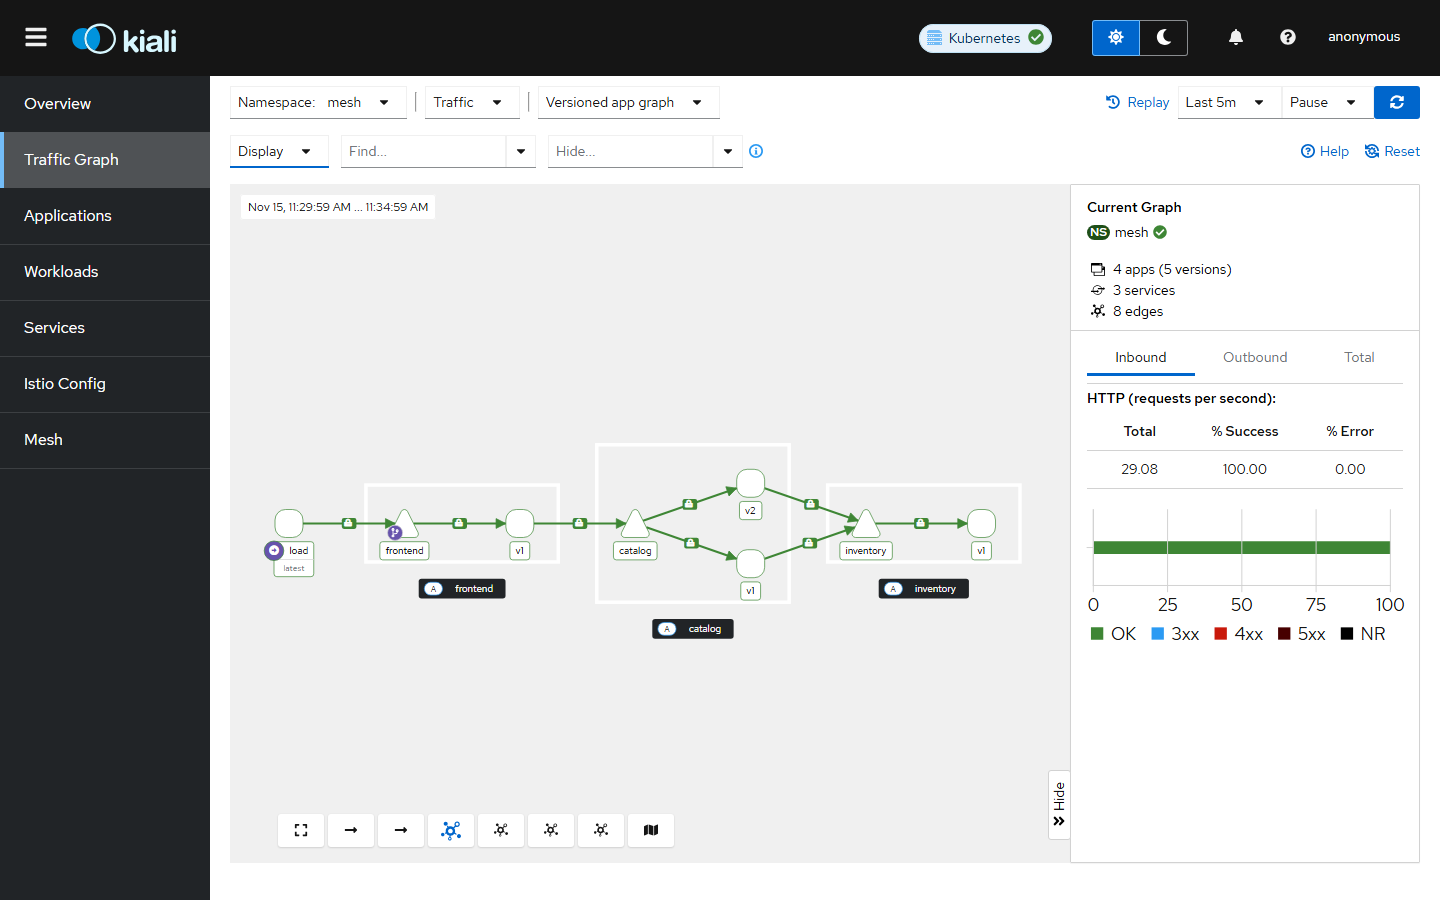
\includegraphics[width=0.9\textwidth]{01-kiali-seguranca.png}
\caption{Kiali: grafo do namespace \texttt{mesh}, com cadeado de mTLS em cada aresta.}
\label{fig:kiali}
\end{figure}

\begin{figure}[ht]
\centering
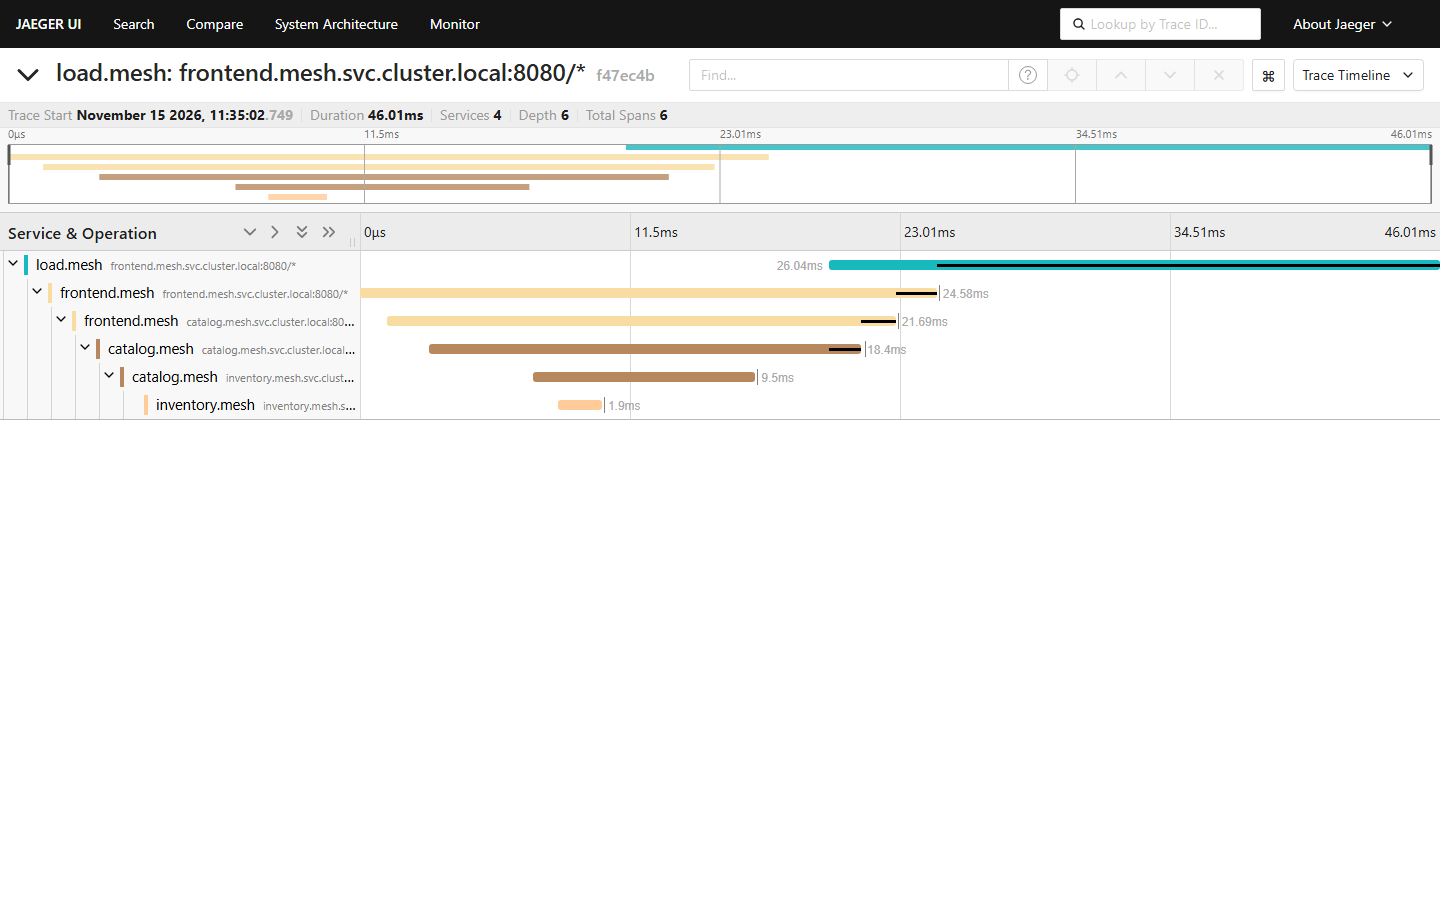
\includegraphics[width=0.9\textwidth]{14-jaeger-trace.png}
\caption{Jaeger: uma requisição com seis \emph{spans} atravessando frontend, catalog e inventory.}
\label{fig:jaeger}
\end{figure}

\subsection{Esforço de implementação}

A Tabela~\ref{tab:loc} conta as linhas (sem comentários nem linhas vazias)
necessárias para obter as mesmas funções. O modo B exigiu 227 linhas, válidas
apenas para serviços em Go e sem rotação de certificados. O modo C exigiu 31
linhas de YAML, válidas para qualquer linguagem, e ainda entrega métricas,
registros e rastreamento sem código adicional.

\begin{table}[ht]
\centering
\caption{Linhas necessárias para as mesmas funções.}
\label{tab:loc}
\small
\begin{tabular}{lrr}
\toprule
Função & B (Go/script) & C (YAML) \\
\midrule
mTLS e autorização por identidade & 46 & 12 \\
Timeout, retry e circuit breaker & 120 & 18 \\
Métricas & 52 & 0 \\
Certificados & 9 & 0 \\
Injeção do sidecar & -- & 1 \\
\midrule
Total & 227 & 31 \\
\bottomrule
\end{tabular}
\end{table}

\section{Discussão}

Para as funções testadas, o Istio deu as mesmas garantias que o código da
aplicação com cerca de sete vezes menos linhas, válidas para qualquer
linguagem, e acrescentou rotação de certificados e observabilidade que o modo B
não tem. O custo apareceu na latência sob concorrência, na memória e na vazão.

Como o mTLS em Go quase não alterou a latência do modo B, o custo do modo C
vem de passar por dois proxies a cada salto e da telemetria que eles geram; a
repetição do teste de vazão com rastreamento em 1\% mostra o peso desta
última. Esses resultados seguem a direção de outros estudos. Zhu et al.
atribuem a maior parte do custo do Envoy ao processamento do protocolo
HTTP~\cite{zhu2023}. Bremler-Barr et al. mediram, com mTLS obrigatório, o maior
aumento de latência no Istio em modo sidecar e o menor no modo
\emph{ambient}~\cite{barr2025}. A documentação do Istio, conforme a versão,
cita de décimos de milissegundo a cerca de 1,5~ms a mais no p90 e no p99 por
salto e de 40 a 60~MB de memória por proxy~\cite{istio-perf}, valores próximos
dos medidos aqui com uma conexão e da memória de cada sidecar (35 a 45~Mi). O
modo \emph{ambient}, estudado no Grau A, substitui os sidecars por um proxy L4
por nó e usa proxies L7 apenas onde são necessários~\cite{istio-ambient}.

Para sistemas com muitos serviços, várias linguagens e exigências de auditoria
e confiança zero, o ganho operacional tende a compensar o custo. Para poucos
serviços sensíveis a latência, as funções na aplicação ou um plano de dados
mais leve podem ser mais adequados.

\section{Limitações}

O cluster é pequeno (três nós de 2 vCPU, limitados pela cota da conta
acadêmica), e os valores absolutos de latência sob concorrência dependem desse
hardware; o que vale é a comparação entre os modos no mesmo ambiente. A causa
exata do aumento de latência com 32 conexões no modo C não foi isolada; a
hipótese mais provável é a disputa de CPU no nó de aplicação, onde ficam os
sidecars. A medição de CPU por \texttt{kubectl top} tem amostragem grosseira.
Foram feitas apenas três rodadas por configuração, com uma única topologia de
três saltos e apenas o modo sidecar. O modo B usa certificados estáticos, sem
rotação, o que o favorece na contagem de linhas. As medições de latência e
recursos do modo C foram feitas com rastreamento em 100\% e registro de acesso
ligados; apenas a vazão foi repetida com a telemetria no padrão, e nela o modo
C melhorou cerca de 75\%.

\section{Conclusão}

Este trabalho implementou, implantou e mediu um protótipo do Istio sobre uma
cadeia de microsserviços em Go no Kubernetes, comparando-o com HTTP puro e com
as mesmas funções escritas na aplicação. O Istio tirou do código o mTLS, a
autorização por identidade, o tempo limite, as retentativas, o circuit breaker
e a observabilidade, com o mesmo efeito medido e muito menos configuração. Em
troca, cobrou em latência sob carga, memória e vazão, custos que vêm dos
proxies e da telemetria; o mTLS em si pesou pouco. Como trabalho futuro,
propõe-se repetir as medições no modo \emph{ambient}, em nós maiores e com a
telemetria no padrão, para separar o custo do proxy, o da telemetria e o da
disputa de CPU.

\bibliographystyle{sbc}
\bibliography{refs}

\end{document}
